\documentclass[11pt,aspectratio=169,usenames,dvipsnames]{beamer}
\usetheme{SimplePlus}

\usepackage{threeparttable}
\usepackage{booktabs}
\usepackage{xcolor} % For custom colors
\usepackage{tikz} % For styling enumerate numbers
\usepackage{tcolorbox} % For colored box styling
\usepackage{amsmath, amsfonts, amssymb, amsthm} % Math related
\usepackage{natbib}
\usepackage{fontspec}
\usepackage{luatexja}
\usepackage[mathscr]{euscript}

% ---------------- %
% color definition %
% ---------------- %
\definecolor{main}{HTML}{23373B}
\definecolor{pink}{RGB}{180, 50, 110}
\definecolor{orange}{HTML}{FF8000}
\definecolor{red}{HTML}{990000}
\definecolor{blue}{HTML}{004C99}
\definecolor{lightgray}{HTML}{E7E7E7}
\definecolor{gray}{RGB}{90, 90, 90}

\newcommand{\pink}[1]{\textcolor{pink}{#1}}
\newcommand{\orange}[1]{\textcolor{orange}{#1}}
\newcommand{\red}[1]{\textcolor{red}{#1}}
\newcommand{\blue}[1]{\textcolor{blue}{#1}}
\newcommand{\green}[1]{\textcolor{OliveGreen}{#1}}
\newcommand{\magenta}[1]{\textcolor{magenta}{#1}}
\newcommand{\gray}[1]{\textcolor{gray}{#1}}
\newcommand{\purple}[1]{\textcolor{purple}{#1}}
\definecolor{yellow}{HTML}{EDB120}

% \setbeamercolor{alerted text}{fg=blue}

%%% automatically add spaces into enumerate and itemize environment
\let\tempone\itemize
\let\temptwo\enditemize
\renewenvironment{itemize}{\tempone\addtolength{\itemsep}{\fill}}{\temptwo}
\let\tempa\enumerate
\let\tempb\endenumerate
\renewenvironment{enumerate}{\tempa\addtolength{\itemsep}{\fill}}{\tempb}

\usepackage{fontawesome5}
\setbeamertemplate{itemize item}{\faAngleRight}
\setbeamertemplate{itemize subitem}{\faAngleDoubleRight}

\setmainfont{Crimson Pro Light}[
  ItalicFont={* Italic},
  BoldFont={Crimson Pro Medium},
  BoldItalicFont={Crimson Pro Medium Italic}]
\setsansfont{Crimson Pro Light}[
  ItalicFont={* Italic},
  BoldFont={Crimson Pro Medium},
  BoldItalicFont={Crimson Pro Medium Italic}]

\usepackage[mode=tex]{standalone}
\usepackage{tikz}
\usetikzlibrary{decorations}
\usetikzlibrary{decorations.pathreplacing, intersections}
\usepackage{pgfplots}
\usetikzlibrary{calc,positioning}
\usepgfplotslibrary{fillbetween}
\pgfplotsset{compat=newest, scale only axis, width = 10cm}

% --------------------------- %
% Section title page with toc %
% --------------------------- %
\setbeamertemplate{subsection page}{%
    \usebeamertemplate*{section page}
}
\setbeamertemplate{section in toc}[square]
\setbeamertemplate{subsection in toc}[square]
\AtBeginSection[]{
% \sepframe
\begin{frame}[noframenumbering]{Outline}
    % \tableofcontents[currentsection]
    \tableofcontents[currentsection, currentsubsection]
\end{frame}
}
\AtBeginSubsection[]{
  \begin{frame}[noframenumbering]{Outline}
    \tableofcontents[currentsection, currentsubsection]
  \end{frame}
}

% ------------ %
% beamerbutton %
% ------------ %
\newcommand{\goto}[2]{\hyperlink{#2}{\beamergotobutton{#1}}}
\newcommand{\return}[2]{\hyperlink{#2}{\beamerreturnbutton{#1}}}
\newcommand{\extgoto}[2]{\href{#2}{\beamergotobutton{#1}}}

\hypersetup{
    pdfpagemode=UseNone,
    pdftitle = {Macroeconomics I, Lecture 5},
    pdfauthor = {Hui-Jun Chen},
    pdfsubject = {},
    pdfkeywords = {},
}

\title[Lecture 5]{Lecture 5 \\ Representative Consumer \\ Optimization and Application}
\author[Hui-Jun Chen]{Hui-Jun Chen}
\institute[NTHU]{National Tsing Hua University}
\date{\today}

\begin{document}

% Title Page
\begin{frame}[plain]
    \titlepage
\end{frame}

\begin{frame}{Overview: Lecture 4 - 7}
\label{slide:Overview__Lecture_4_7}

\begin{center}
Provide \alert{micro-foundation} for the \alert{macro implication} (\alert{Lucas critique})
\end{center}

\begin{itemize}
    \item \textbf{Representative Consumer}:
    \begin{itemize}
        \item Lecture 4: \alert{preference}, \alert{constraints}
        \item Lecture 5: \alert{optimization}, \alert{application}
        \item Lecture 6: Numerical Examples
    \end{itemize}
    \item \textbf{Representative Firm}:
    \begin{itemize}
        \item Lecture 7: \alert{production}, \alert{optimization}, \alert{application}
    \end{itemize}
\end{itemize}
\end{frame}

\begin{frame}{Review: MRS}
\label{slide:Review__MRS}
    \begin{columns}
        \begin{column}{0.5\textwidth}
            \begin{itemize}
                \item \alert{Normality}: M{\tiny arginal}R{\tiny ate of }S{\tiny ubstitution}
                \begin{itemize}
                    \item \textbf{Marginal}: for \alert{arbitrary small} change in $ x $-axis (leisure in this case)
                    \item \textbf{rate of substitution}: the amount on $ y $-axis has to be sacrificed (consumption in this case)
                \end{itemize}
                %
                \begin{equation}
                \label{eq:MRS}
                    MRS_{l, C} = \frac{D_{l} U( C, l )}{D_{C}U( C, l )}
                ,\end{equation}
                %
                where $ D_{x}U( \cdot ) $ is derivative of $ U $ w.r.t. $ x $
            \end{itemize}
        \end{column}
        \begin{column}{0.5\textwidth}
        \begin{figure}
            \caption{Figure 4.2 MRS}
            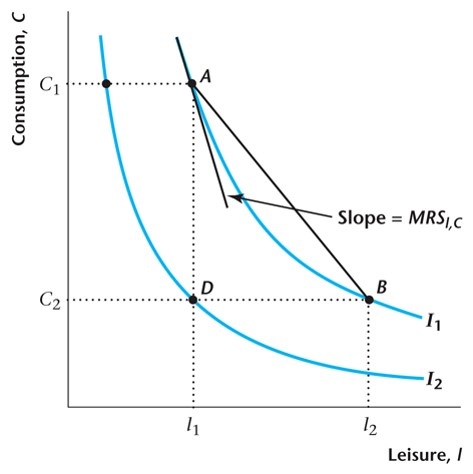
\includegraphics[width=.8\textwidth]{./figures/Figure4_2.jpg}
        \end{figure}
        \end{column}
    \end{columns}
\end{frame}

\section{Optimization}
\label{sec:Optimization}

\begin{frame}{Consumer's Problem}
\label{slide:Consumer_s_Problem}
    The consumer choose \alert{consumption} and \alert{leisure} bundle to achieve \alert{highest} indifference curve, while still satisfying \alert{budget constraint}
     %
     \begin{equation}
     \label{eq:HHProblem}
         \begin{split}
             \max_{C, l} \quad
                 & U( C, l )
             \\
             \text{subject to } \quad
                & C \le w( h - l ) + \pi - T
            \\
         \end{split}
     \end{equation}
     %
     \begin{itemize}
         \item \textbf{Rational behavior}: decision is made given preference \& constraints
         \item \textbf{Analysis}: both \alert{graphically} and \alert{algebraically}
     \end{itemize}
\end{frame}

\begin{frame}{Graphical Analysis: Interior Solution}
\label{slide:Graphical_Analysis__Interior_Solution}
    \begin{columns}
        \begin{column}{0.5\textwidth}
            \begin{itemize}
                \item \textbf{Interior}: sol. at middle of budget set, not end pts
                \item \alert{MRS} must equal to \alert{real wage} ($MRS_{l, C} = w$), WHY?
                \begin{itemize}
                    \item sacrificed consumption comes from the decrease of labor income
                \end{itemize}
                \item Sol. at indifference curve \alert{tangent} to budget set
                \item \textbf{Convexity}: E v.s. H \& F v.s. H
            \end{itemize}
        \end{column}
        \begin{column}{0.5\textwidth}
            \begin{figure}
                \caption{Figure 4.5 Interior Solution}
                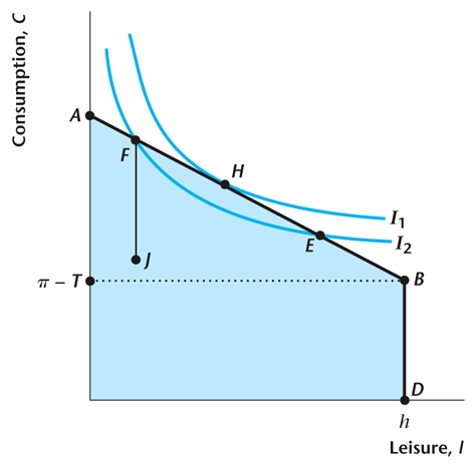
\includegraphics[width=.8\textwidth]{./figures/Figure4_5.jpg}
            \end{figure}
        \end{column}
    \end{columns}
\end{frame}

\begin{frame}{Graphical Analysis: Corner Solution}
\label{slide:Graphical_Analysis__Corner_Solution}
    \begin{columns}
        \begin{column}{0.5\textwidth}
            \begin{itemize}
                \item \textbf{Corner}: sol. at end pts of budget set
                \item \alert{MRS} \alert{NOT} equal to \alert{real wage} ($MRS_{l, C} \neq w$), WHY?
                \begin{itemize}
                    \item working limited to total $ h $ hours, ``kink''
                \end{itemize}
                \item Sol. is NOT tangent to indifference curve
                % \item \textbf{Convexity}: E v.s. H \& F v.s. H
            \end{itemize}
        \end{column}
        \begin{column}{0.5\textwidth}
            \begin{figure}
                \caption{Figure 4.6 Corner Solution}
                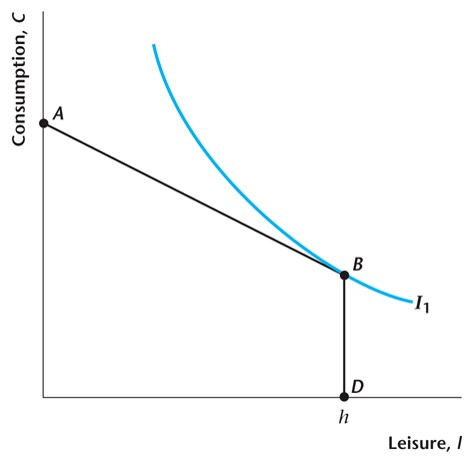
\includegraphics[width=.8\textwidth]{./figures/Figure4_6.jpg}
            \end{figure}
        \end{column}
    \end{columns}

\end{frame}

\begin{frame}{Algebraic Analysis: Interior Solution}
\label{slide:Algebraic_Analysis__Interior_Solution}
    Recall consumer's problem:
    %
    \begin{equation}
    \label{eq:HHProblem_recall}
        \begin{split}
            \max_{C, l} \quad
                & U( C, l )
            \\
            \text{subject to } \quad
               & C \le w( h - l ) + \pi - T
           \\
        \end{split}
    \end{equation}
    %
    \begin{itemize}
        \item Calculus is about \alert{derivative}: not defined at ``kink'' $ \Rightarrow  $ only \alert{interior sol.}
        \item Sol. at the \alert{border} of budget set $ \Rightarrow  $ budget constraint is ``$ = $'' (\alert{binding})
    \end{itemize}
    Plug the budget constraint into utility function to replace $ C $, we get
    %
    \begin{equation}
    \label{eq:HHProblem_plugin}
        \max_{l} \quad U( w( h-l ) + \pi - T, l )
    \end{equation}
    %
\end{frame}

\begin{frame}{Algebraic Analysis: Interior Solution (Cont.)}
\label{slide:Algebraic_Analysis__Interior_Solution__Cont__}
    %
    \begin{equation*}
        \max_{l} \quad U( w( h-l ) + \pi - T, l )
    \end{equation*}
    %
    Remember that now $ C = w( h-l ) + \pi - T $.
    Take \alert{first order condition} w.r.t. $ l $,
    %
    \begin{align}
        \overbrace{D_{C} U( C, l ) \times \frac{d [ w ( h-l ) + \pi - T ]}{d l}}^{\text{Derivative on $ C $ direction, \goto{chain rule}{slide:Chain_rule}}}
            & + \overbrace{D_{l} U( C, l )}^{\text{Derivative on $ l $ direction}} = 0
        \\
        D_{C}U( C, l ) \times ( -w )
            & + D_{l} U( C, l ) = 0
        \\
        w = \frac{D_{l}U( C, l )}{D_{C}U( C, l )}
            & = MRS_{l, C}
    \end{align}
    %
    Note: $ D_{x} f( \cdot ) $ is a shorthand for $ \frac{d f( \cdot )}{d x} $, meaning \alert{differentiation} of $ f( \cdot ) $ with respect to choice variable $ x $.
\end{frame}

\section{Experiment}
\label{sec:Experiment}

\begin{frame}{Build model for experiment}
\label{slide:Build_model_for_experiment}
    \begin{itemize}
        % \item Macroeconomists usually \textbf{cannot} do experiment: severe impact
        \item We want to know \alert{what's the result of changes}!
        \item Recall \alert{Lucas critique}: need to understand individual behavior
        \item Consider two experiments:
        \begin{enumerate}
            \item direct increase in \alert{real income} (no $ C $ and $ l $ trade off, pure \alert{income effect})
            \item increase in \alert{real wage} (\alert{income + substitution effect})
        \end{enumerate}
    \end{itemize}
\end{frame}

\begin{frame}{Experiment 1: Increase in dividends / Decrease in Tax}
\label{slide:Experiment_1__Increase_in_dividends}
    \begin{columns}
        \begin{column}{0.5\textwidth}
            \begin{itemize}
                \item \textbf{Recall}: $ C $ \& $ l $ are normal goods
                \item \textbf{Income effect}: income $ \uparrow  $ $ \Rightarrow  $ normal goods $ \uparrow  $
                \item Increase in dividends or decrease in taxes are level shifts up in real income, regardless of actions
                \item Consumer increases consumption, reduces quantity of labor supplied (increase leisure).
            \end{itemize}
        \end{column}
        \begin{column}{0.5\textwidth}
            \begin{figure}
                \caption{Figure 4.6 $ \pi \uparrow $ / $ T \downarrow  $}
                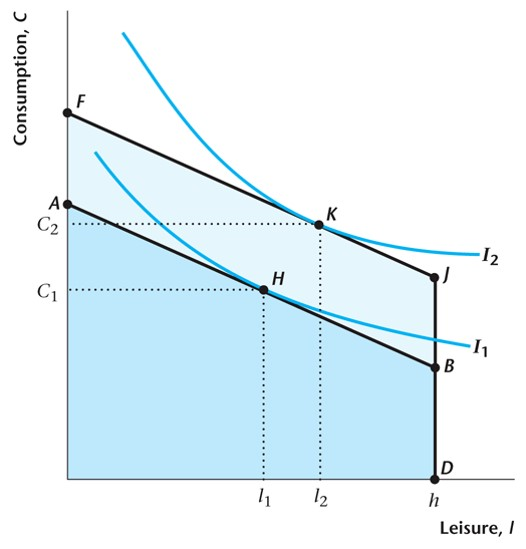
\includegraphics[width=.8\textwidth]{./figures/Figure4_7.jpg}
            \end{figure}
        \end{column}
    \end{columns}
\end{frame}

\begin{frame}{Experiment 2: Increase in Real Wage}
\label{slide:Experiment_2__Increase_in_Real_Wage}

    \begin{columns}
        \begin{column}{0.5\textwidth}
            \textbf{Substitution effect}: $ w \uparrow  $, leisure is costly, sacrifice $ l $ for $ C $
            \begin{itemize}
                \item budget line AB to JK, keeps F just affordable
                \item move along $ I_{1} $ : new slope of budget line
            \end{itemize}
            \textbf{Income effect}: income $ \uparrow  $ $ \Rightarrow  $ normal goods $ \uparrow  $
            \begin{itemize}
                \item budget line JK to EB, actual new budget line
                \item move up to $ I_{2} $: higher utility possible
            \end{itemize}
        \end{column}
        \begin{column}{0.5\textwidth}
            \begin{figure}
                \caption{Figure 4.8  $w \uparrow $, both effects canceled out}
                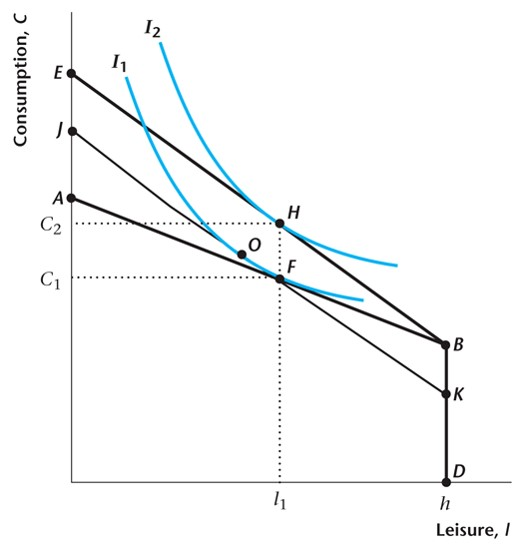
\includegraphics[width=.8\textwidth]{./figures/Figure4_8.jpg}
            \end{figure}
        \end{column}
    \end{columns}

\end{frame}

\begin{frame}{Experiment 1 \& 2: Labor Supply}
\label{slide:Experiment_1____2__Labor_Supply}

    \begin{columns}
        \begin{column}{0.5\textwidth}
        Looking ahead to putting the pieces together in a full model:
        \begin{itemize}
            \item Solution to consumer problem defines the supply curve for the labor market!
            \item What assumption ensures this is increasing in the wage?
            \begin{itemize}
                \item substitution effect: $ w \uparrow \Rightarrow l \downarrow (\text{i.e., } N^{S} \uparrow ) $
                \item income effect: $ w \uparrow \Rightarrow l \uparrow  (\text{i.e., } N^{S} \downarrow ) $
                \item Income effect $ < $ substitution effect
            \end{itemize}
        \end{itemize}
        \end{column}
        \begin{column}{0.5\textwidth}
            \begin{figure}
                \caption{Figure 4.10, LS on $ \pi \uparrow $ / $ T \downarrow  $}
                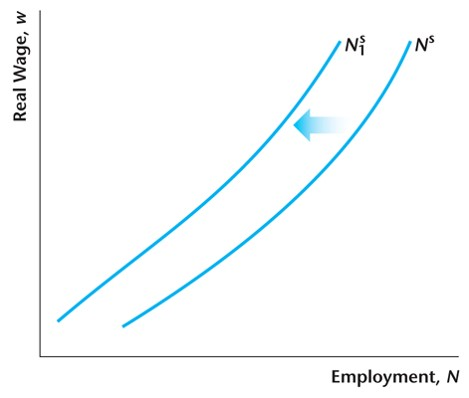
\includegraphics[width=\textwidth]{./figures/Figure4_10.jpg}
            \end{figure}
        \end{column}
    \end{columns}
\end{frame}

\section{Appendix}
\label{sec:Appendix}

\appendix
% -------------------------------------------
\setbeamertemplate{headline}
{
\setbeamercolor{section in head/foot}{fg=black, bg=white}
\vskip1em \tiny \insertsectionnavigationhorizontal{1\paperwidth}{\hspace{0.50\paperwidth}}{}
}
%------------------------------------------
\begin{frame}\frametitle{}
\begin{columns}
\label{Appendix}
\column{1\linewidth}
\centering
{\Large \alert{Appendix}}
\end{columns}
\end{frame}
%------------------------------------------

\begin{frame}{Chain rule}
\label{slide:Chain_rule}
\framesubtitle{\jump{slide:Algebraic_Analysis__Interior_Solution__Cont__}{Back}}
In the main slide, we applied \alert{chain rule} to the $ C $ direction of the $ U( C, l ) $. By binding budget constraints, we know $ C( l ) = w( h-l ) + \pi - T $, i.e., consumption is a function of leisure.

%
\begin{equation}
\label{eq:Chain rule}
    \frac{d}{dl} U( C( l ) ) = \frac{dU( C, l )}{dC} \times \frac{dC( l )}{dl} = D_{C} U( C, l ) \times D_{l} C( l )
\end{equation}
%
where $ D_{l}C( l ) = -w $.

\end{frame}

\end{document}
